\documentclass[12pt,a4paper]{amsart}
% ukazi za delo s slovenscino -- izberi kodiranje, ki ti ustreza
\usepackage[slovene]{babel}
\usepackage[utf8]{inputenc}
%\usepackage[T1]{fontenc}
\usepackage{amsmath,amssymb,amsfonts}
\usepackage{url}
%\usepackage[normalem]{ulem}
\usepackage[dvipsnames,usenames]{color}
\usepackage{caption}
\usepackage{lipsum}
\usepackage{tikz}

\usetikzlibrary{graphs}
\usetikzlibrary{graphs.standard}

%\makeatletter
%\renewcommand\section{\@startsection{section}{1}%
%  \z@{.5\linespacing\@plus.7\linespacing}{.5\linespacing}%
%  {\normalfont\scshape\large\centering}}
%\renewcommand\subsection{\@startsection{subsection}{2}%
%  \z@{.5\linespacing\@plus.7\linespacing}{.5\linespacing}%
%  {\normalfont\scshape}}
%\renewcommand\subsubsection{\@startsection{subsubsection}{3}%
%  \z@{.5\linespacing\@plus.7\linespacing}{-.5em}%
%  {\normalfont\itshape}}
%\makeatother

% ne spreminjaj podatkov, ki vplivajo na obliko strani
\textwidth 15cm
\textheight 24cm
\oddsidemargin.5cm
\evensidemargin.5cm
\topmargin-5mm
\addtolength{\footskip}{10pt}
\pagestyle{plain}
\overfullrule=15pt % oznaci predlogo vrstico


% ukazi za matematicna okolja
\theoremstyle{definition} % tekst napisan pokoncno
\newtheorem{definicija}{Definition}[section]
\newtheorem{primer}[definicija]{Example}
\newtheorem{opomba}[definicija]{Remark}

\renewcommand\endprimer{\hfill$\diamondsuit$}

\theoremstyle{plain} % tekst napisan posevno
\newtheorem{lema}[definicija]{Lemma}
\newtheorem{izrek}[definicija]{Theorem}
\newtheorem{trditev}[definicija]{Statement}
\newtheorem{posledica}[definicija]{Corollary}
\newtheorem{conjecture}[definicija]{Conjecture}


% za stevilske mnozice uporabi naslednje simbole
\newcommand{\R}{\mathbb R}
\newcommand{\N}{\mathbb N}
\newcommand{\Z}{\mathbb Z}
\newcommand{\C}{\mathbb C}
\newcommand{\Q}{\mathbb Q}

% ukaz za slovarsko geslo
\newlength{\odstavek}
\setlength{\odstavek}{\parindent}
\newcommand{\geslo}[2]{\noindent\textbf{#1}\hspace*{3mm}\hangindent=\parindent\hangafter=1 #2}

% naslednje ukaze ustrezno popravi
\newcommand{\program}{Financial mathematics} % ime studijskega programa: Matematika/Finančna matematika
\newcommand{\imeavtorja}{Anej Rozman, Tanja Luštrek} % ime avtorja
\newcommand{\imementorja}{Assistant Professor Janoš Vidali} % akademski naziv in ime mentorja
\newcommand{\imesomentorja}{Professor Riste Škrekovski}
\newcommand{\naslovdela}{Rich-Neighbor Edge Colorings}
\newcommand{\letnica}{2023} %letnica diplome

\begin{document}

\thispagestyle{empty}
\noindent{\large
UNIVERSITY OF LJUBLJANA\\[1mm]
FACULTY OF MATHEMATICS AND PHYSICS\\[5mm]
\program\ -- 1st cycle}
\vfill

\begin{center}{\large
\imeavtorja\\[2mm]
{\bf \naslovdela}\\[10mm]
Term Paper in Finance Lab\\[2mm]
Short Presentation\\[1cm]
Advisers: \imementorja, \imesomentorja\\[2mm]}
\end{center}
\vfill

\noindent{\large
Ljubljana, \letnica}
\pagebreak

\section{Introduction}

In this paper we set out to analyse an open conjecture in a modern graph theory problem known as rich-neighbor edge coloring.


\begin{definicija}
    In an edge coloring, an edge $e$ is called $rich$ if all edges adjacent to $e$ have different colors. An edge coloring is 
    called a $rich\text{-}neighbor \ edge \ coloring$ if every edge is adjacent to some rich edge.
\end{definicija}

\begin{definicija}
    $X'_{rn}(G)$ denotes the smallest number of colors for which there exists a rich-neighbor edge coloring.
\end{definicija}

\begin{conjecture}
    For every graph $G$ of maximum degree $\Delta$, $X'_{rn}(G) \leq 2\Delta - 1$ holds.
\end{conjecture}

\begin{primer}
    Let's take a look at the Petersen graph and an example of a rich-neighbor edge coloring.
    \begin{center}
        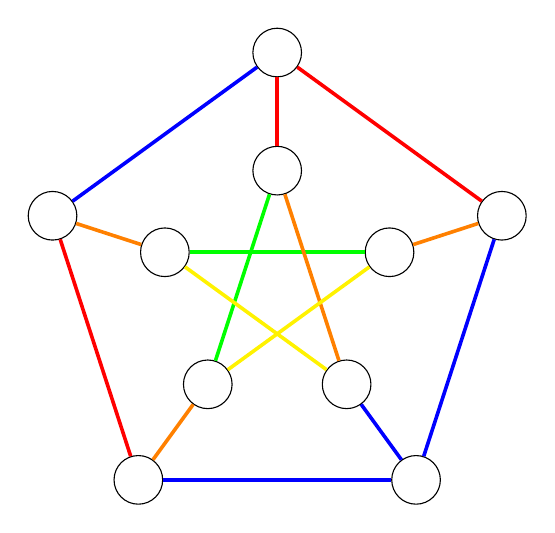
\begin{tikzpicture}[every node/.style={draw,circle, style={text opacity=0}}]
            \graph[clockwise, radius=3cm] {subgraph C_n [n=5,name=A] };
            \graph[clockwise, radius=1.5cm] {subgraph I_n [n=5,name=B] };
    
    
            % Define edge colors for the graph
            \draw[red, line width=1.3pt] (A 1) -- (B 1);
            \draw[orange, line width=1.3pt] (A 2) -- (B 2);
            \draw[blue, line width=1.3pt] (A 3) -- (B 3);
            \draw[orange, line width=1.3pt] (A 4) -- (B 4);
            \draw[orange, line width=1.3pt] (A 5) -- (B 5);
            \draw[red, line width=1.3pt] (A 1) -- (A 2);
            \draw[blue, line width=1.3pt] (A 2) -- (A 3);
            \draw[blue, line width=1.3pt] (A 3) -- (A 4);
            \draw[red, line width=1.3pt] (A 4) -- (A 5);
            \draw[blue, line width=1.3pt] (A 5) -- (A 1);
            \draw[green, line width=1.3pt] (B 5) -- (B 2);
            \draw[green, line width=1.3pt] (B 4) -- (B 1);
            \draw[orange, line width=1.3pt] (B 3) -- (B 1);
            \draw[yellow, line width=1.3pt] (B 5) -- (B 3);
            \draw[yellow, line width=1.3pt] (B 4) -- (B 2);
        \end{tikzpicture}
    \end{center}
    We can see that for the Petersen graph (which is 3-regular) $X'_{rn}=5 \leq 5$.
\end{primer}

\section{Plan}
Our assingnment is to create an algorthm that proves the conjecture for graphs of maximum degree 4 (So it finds a rich-neighbor edge coloring for every graph, for example for all graphs with 5 veriticies and a maximum degree of 5), and to make a random search algorythm for graphs of maximum degree $\geq5$.


\end{document}